\chapter{Standard Model}

\label{ch:standardmodel}
% --------------------------------------------------------------------------------

%\section{Particles}
%\label{sec:particles}
%
\section{Action and the Lagrangian}

Originally, both action and the Lagrangian were constructed for an integral reformulation of the laws of classical mechanics, which is a purely mathematical step: any differential equation can be re-expressed in terms of an integral equation. 
The Lagrangian, $\mL$, is classically given by the difference of  kinetic energy and potential energy. 
The Lagrangian is defined this way so that the action, $\mS$, given by 
\begin{equation}\label{eq:action}
 \mS[\vect{q}(t)] = \int_{t_1}^{t_2} \mL(\vect{q},\dot{\vect{q}},t)\ dt
\end{equation}
\noindent returns the classical equations of motion when one requires it to be stationary in the path, $\vect{q}(t)$. 
This formulation of classical mechanics is extremely useful in calculations, and generalizes beautifully to cover all types of physics.

In particular, with the development of quantum mechanics in the twentieth century, the concepts of action and the Lagrangian were found to generalize to more complicated physics for which the classical laws do not hold. 
Quantum mechanics and quantum field theory can be constructed from the action, using the path integral formulation, by assuming that a particle undergoes all possible paths $\vect{q}(t)$ with an imaginary phase given by $e^{i \mS[\vect{q}(t)]/\hbar}$. 
This reduces to classical mechanics in the limit as $\hbar$ goes to zero, as all paths for which the action is not stationary interfere with each other so as to cancel their contributions. 
Because the  wavefunction of a particle can be completely determined through the action and the action depends only on the Lagrangian, the Lagrangian itself is sufficient to describe the physics governing the particle. 

So, in both classical and quantum mechanics, the Lagrangian of a system contains everything there is to know about the system, apart from initial conditions. 
Thus, the most natural way to express that a system has a certain symmetry is to require that the Lagrangian is invariant under a corresponding symmetry transformation. 
This makes the Lagrangian the central  piece of the discussion of gauge invariance; the mathematical representation of gauge invariance is that a gauge transformation on the appropriate components of the Lagrangian  returns an identical Lagrangian. That is,

\begin{align}
\mL(\psi,D^{\mu}) = \mL(U\psi, D^{'\mu})
\end{align}

\noindent where $\psi$ is the wavefunction and $D^{\mu}$ is the covariant derivative, both of which transform under a symmetry operation.
There are a number of immediate and suprisingly powerful consequences of requiring that the Lagrangian is invariant under a symmetry operation.

\section{Gauge Invariance and Forces}

The simplest possible Lagrangian is the free Dirac Lagrangian, which describes a relativistic fermion in a vacuum.

\begin{align}\label{eq:free_dirac} 
\mL = i\bar{\psi}\slashed{\partial}\psi -m\bar{\psi}\psi 
\end{align}

\noindent A fermion denotes a particle with spin-1/2, and the kinematic term in the Lagrangian correctly describes the free propagation of a fermionic particle with mass $m$. 
This equation is clearly invariant under a global $U(1)$ transformation, that is changing $\psi$ by a complex phase has no effect. 
The derivative operator commutes with a constant phase factor, and wherever $\psi$ appears it's complex conjugate also appears so as to cancel out the change of phase. 
However, the Lagrangian as written is not invariant under the local $U(1)$ symmetry postulated for the \ac{SM}, which can be written as $U = e^{i\alpha(x)}$. 
The piece of the Lagrangian involving a derivative will return an extra term that will break the invariance of the Lagrangian under this transformation:

\begin{align*}
 \mL' &= i (\bar{\psi}U^\dagger)\slashed{\partial}(U\psi) - m(\psi U^\dagger)(U\psi) \\
      &= i (\bar{\psi}U^\dagger) U(\slashed{\partial} - \gamma^\mu \partial_\mu\alpha(x))\psi - m(\psi U^\dagger)(U\psi) \\
      &= i \bar{\psi}\slashed{\partial}\psi -m\bar{\psi}\psi - i\gamma^\mu \partial_\mu\alpha(x)\bar{\psi}\psi  \\
      &= \mL -  i\gamma^\mu \partial_\mu\alpha(x)\bar{\psi}\psi \\
      &\neq \mL 
\end{align*}

\noindent So, in order to enforce the required symmetry, the typical approach is to construct a covariant derivative, that is to add a term to the derivative operator so that the unwanted term in $\mL'$ is exactly cancelled. 
A generic form for such a derivative is given by

\[ D^\mu = \partial^{\mu} - iqA^\mu \]

\noindent where at this point $A^\mu$ is an arbitrary field that transforms under the $U(1)$ operator and $q$ is a scaling factor. Adding this component to the above Lagrangian gives

\begin{align}
 \mL' &=  i (\bar{\psi}U^\dagger) U(\slashed{\partial} - \gamma^\mu \partial_\mu\alpha(x) - iq\gamma^\mu A'_{\mu})\psi - m(\psi U^\dagger)(U\psi) \\
 \mL' &= \mL +\gamma^\mu (- i\partial_\mu\alpha(x) - iqA'_{\mu} + iqA_\mu)\bar{\psi}\psi 
\end{align}

\noindent and because the transformation of $A^\mu$ is unspecified, we will have that $\mL = \mL'$ whenever

\[  A'_\mu =  A_{\mu} - \frac{1}{q}\partial_\mu\alpha(x) \]

The above procedure demonstrated that beginning with the Lagrangian for a free fermion and imposing a local $U(1)$ symmetry required the existence of a vector field $A^\mu$, and specified it's tranformation under the $U(1)$ gauge group.
The additional term in the derivative can expanded to form a completely separate term in the Lagrangian,

\begin{align}
\mL = i\bar{\psi}\slashed{\partial}\psi -m\bar{\psi}\psi - (q\bar{\psi}\gamma^\mu\psi)A^\mu
\end{align}

\noindent and in this form it is clear that the $A^\mu$ term has the exact form of the electromagnetic interaction.
That is, this is the Lagrangian which reproduces the relativistic form of Maxwell's equations for a particle interacting with an electromagnetic field.
It is natural to also introduce a term to the Lagrangian at this point to describe the free propagation of the vector $A$ field, where the propagation of a vector field has the form of

\begin{align}
- \frac{1}{16\pi} F^{\mu\nu}F_{\mu\nu} \quad \mathrm{with} \quad F_{\mu\nu} = \partial_\mu A_\nu - \partial_\nu A_\mu
\end{align}

\noindent which then also describes the electromagnetic interactions in a vacuum and the propogation of a photon.
The photon is an example of a gauge boson, a spin-0 particle required to exist by a gauge symmetry of the Lagrangian and one that corresponds to a force.
In summary, requiring the $U(1)$ symmetry was enough to recover all of electromagnetism and to predict the existence of a photon in the \ac{SM}. 

The interaction term that was placed into the Lagrangian by this procedure can be conveniently summarized with Feynman diagrams, which diagramatically represent a transition from an initial state to a final state.
All diagrams that start with the same initial state and end with the same final state must be considered, but more complicated diagrams can be built by linking together the simplest versions.
A diagram that corresponds to the above term, $(q\bar{\psi}\gamma^\mu\psi)A^\mu$, is shown in Figure~\ref{fig:feyn_aff}, for an interaction with a generic fermion.

\begin{figure}
%\includegraphics[width=\fullfig]{}
\caption{A Feynman diagraming representing the interaction of the $A$ field with a generic fermion, $f$.} 
\label{fig:feyn_aff}
\end{figure}


\subsection{$SU(2)\times U(1)$ and the Electroweak Force}

The full picture of the electroweak section of the \ac{SM} is more complicated than the simplified explanation of the electromagnetic piece described above. 
In practice, it is necessary to consider the entire $SU(2)\times U(1)$ symmetry together, but the procedure is the same.
Enforcing the symmetry on the Lagrangian requires the introduction of a covariant derivative, this time with four total distinct terms, one for each of the generators of $SU(2)\times U(1)$.
The result is a series of terms in the Lagrangian which describe the interaction of a fermion with four vector fields, the $W_1$, $W_2$, $W_3$, and $B$ fields.
These fields can mix in the quantum sense, and linear combinations form the $W^+$, $W^-$, $Z$, and $A$ fields that are considered actual particles in the \ac{SM}\footnote{These states are the actual particles because they are mass eigenstates, but the full explanation of this will have to wait for the discussion of the Higgs mechanism.}.
The interactions between these fields and fermions are summarized in Figure~\ref{fig:feyn_electroweak}.

\begin{figure}
%\includegraphics[width=\fullfig]{}
\caption{The interactions of the electroweak gauge bosons with generic fermions.} 
\label{fig:feyn_electroweak}
\end{figure}

\subsection{$SU(3)$ and the Strong Force}

The same procedure can be applied starting with the $SU(3)$ symmetry requirement, where eight additional fields must be introduced, one for each of the generators of $SU(3)$.
The resulting Lagrangian describes \ac{QCD} and predicts the existence of eight gauge bosons known collectively as gluons. 
The interactions between these fields and fermions are summarized in Figure~\ref{fig:feyn_strong}.

\begin{figure}
%\includegraphics[width=\fullfig]{}
\caption{The interaction of the strong gauge bosons, the gluons, with generic fermions.} 
\label{fig:feyn_strong}
\end{figure}


\section{Noether's Theorem, Charges, and Matter}

Another direct consequence of the symmetries stipulated in the \ac{SM} are a series of conserved quantities, Noether charges, named after the mathemetician and physicst Emmy Noether.
The charges arise as a direct consequence of Noether's theorem, which can be informally stated as 
\begin{quote}
\textit{For every symmetry of the Lagrangian, there exists a corresponding physical quantity whose value is conserved in time.}
\end{quote}
\noindent Or, stated another way, symmetries of the Lagrangian mathematically require the conservation of specific quantities taken from the Lagrangian. 
This relationship can also be thought of as operating in the other direction, the existence of a conserved charge can be shown to generate the symmetry in the Lagrangian.
This theorem is actually quite striking in a somewhat unexpected relation between simple geometric symmetries and physically observable conservation laws. 
For example, the theorem connects the translation invariance of the Lagrangian in space to the conservation of momentum and the translation invariance in time to the conservation of energy. 

\textbf{Quick derivation of conservation of charge here.}

In the context of the \ac{SM}, the required symmetries of $U(1)\times SU(2) \times SU(3)$ correspond to the charges that are considered properties of all elementary particles.
The most familiar of these properties is the electric charge, Q, which is one of the conserved quantities of $SU(2)\times U(1)$.
The remaining pieces of $SU(2)\times U(1)$ correspond to weak isospin, $T$ and $T_3$, where $T$ has only non-negative values and $T_3$ can be positive and negative.
The $SU(3)$ symmetry is generated by the three colors of \ac{QCD}, red, green, and blue, each with a corresponding opposite color, anti-red, anti-green, and anti-blue.

The matter in the observable universe consists of a collection of particles which carry these charges, in addition to spin and mass.
The particles typically thought of as matter are all fermions: particles with spin-1/2.
All of the fermions belong to one of two groups, quarks and leptons, and one of three generations.
Each of the generations have similar properties but significantly different masses; the particles in consecutive generations have increasing mass.
Quarks are distinquished from leptons in that they carry color charge, in addition to  electric charge and weak isospin.
The particles in the \ac{SM} are summarized in Figure~\ref{fig:particle_content}, and the matter particles are the twelve types of fermions displayed on the left side of the graphic.

\begin{figure}[h]
  \centering
  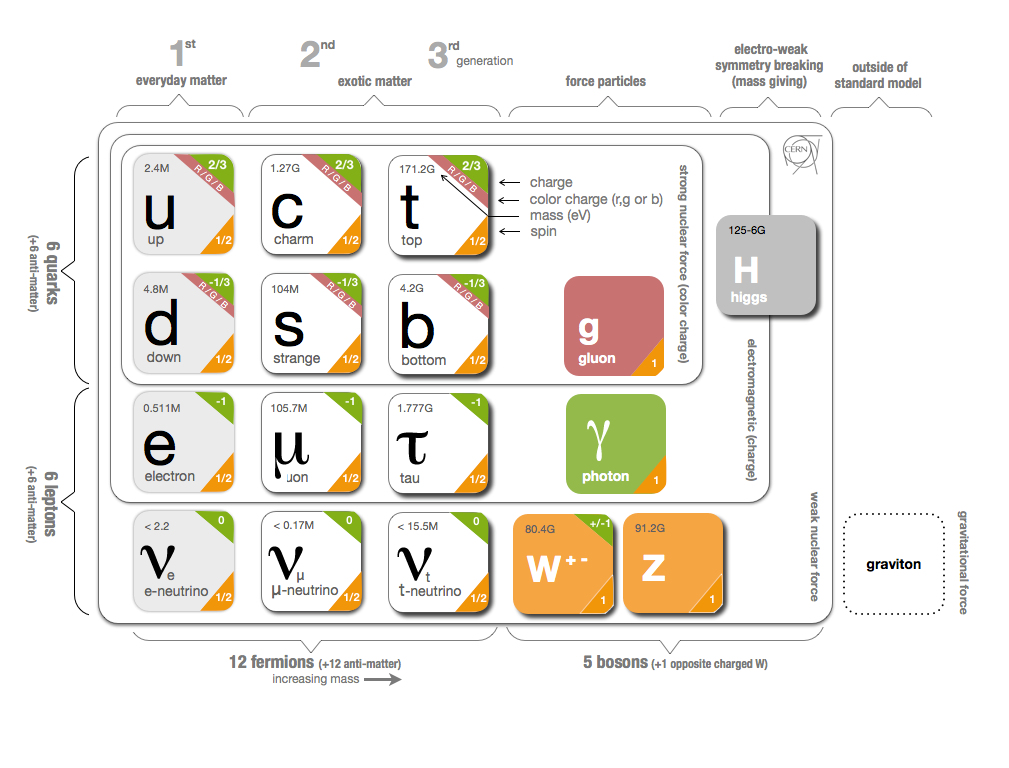
\includegraphics[width=0.9\textwidth]{figures/particle_content.png}
  \caption{The particle content of the \ac{SM}.}
  \label{fig:particle_content}
\end{figure}


\subsection{Quarks}

The three generations of quarks each have a particle with electric charge $+2/3$ and one with charge $-1/3$.
They are referred to us up and down, charm and strange, and top and bottom respectively, and these are referred to as the quark flavors.
Although Figure~\ref{fig:particle_content} only shows these six flavors, there is a unique particle for each combination of the three colors and flavor.
And each quark has an anti-particle with the opposite electric and color charge values.

However, individual quarks are never observed in nature, but instead form color-neutral bound states.
One way to form a color neutral combination is a bound state of three quarks with three different color charges, called a baryon.
Baryons are the most common type of quark configuration in conventional matter, and include protons and neutrons.
The other common configuration is a bound state of a quark and an anti-quark, called a meson, where the two quarks have the same type but opposite colors. 
The conservation of the various charges carried by quarks, along with the requirement that quarks appear in color-neutral states, result in the observed conservation of baryon number, $B$, where baryons have $B=1$ and mesons have $B=0$. 

\subsection{Leptons}

The remaining fermions, the leptons, do not carry color charge.
Each generation contains an electrically charged lepton, the electron, muon, and tau, and an electrically neutral lepton called a neutrino.
For the charged leptons, the flavors are mass eigenstates, with the masses listed in Figure~\ref{fig:particle_content}.
The flavors of the neutrinos, on the other hand, are not mass eigenstates: they propagate in mass eigenstates and so can oscillate between different flavors.
The absolute masses of the neutrinos are not currently known, but the phenomenon of oscillations shows that they have three different mass values.
Although there is no direct conservation law resulting from the symmetries of the \ac{SM} Lagrangian, no interactions have been observe which alter lepton number, $L$, the difference in the number of leptons and anti-leptons. 

\subsection{Chirality}

All of the fermions described above have two possible values of the magnitude of weak isospin, $T$, either $0$ or $1/2$.
The fermions with $T = 0$ are called right-handed, while those with $T=1/2$ are called left-handed.
For left-handed fermions, each of the quark and lepton generations have one particle with $T_3 = -1/2$ and one with $T_3 = +1/2$.
The neutrinos have $T_3 = +1/2$, while the charged leptons have $T_3 = -1/2$.
Similarly, the positively charged quarks have $T_3 = +1/2$ and the negatively charged quarks have $T_3 = -1/2$.
Because the right-handed neutrinos would have no charge of any type, it is not clear if they exist at all.


\section{Higgs Mechanism and Mass}

\section{Phenomenology}



% --------------------------------------------------------------------------------
% Old Intro

%The \ac{SM} of particle physics seeks to explain the symmetries and interactions of fundamental particles. 
%The \ac{SM} provides predictions in particle physics for interactions up to the Planck scale (10\tsup{15}-10\tsup{19} \GeV).
%It has been tested by several generations of experiments and has been remarkably succesful; no significant deviations from its predictions have been found.
%
%The theory itself is a quantum field theory grown from an underlying symmetry, $SU(3) \times SU(2) \times U(1)$, that generates all of the interactions consistent with experimental observations.
%Each postulated symmetry necessitates the existance of an associated conserved charge, through Noether's theorem, which appear as properties of the observed particles in nature. 
%These interactions are referred to as the Strong, Weak, and Electromagnetic forces, which are discussed in Section~\ref{sec:interactions}. 
%
%Although this model has been very predictive, the theory is incomplete; for example, it is not able to describe gravity or astronomically observed dark matter. 
%These limitations are discussed in more detail in Section~\ref{sec:limitations}. 
%


% Old section on particles, before the redesign
%\section{Particles}
%\label{sec:particles}
%
%The most familiar matter in the universe is made up of protons, neutrons, and electrons. 
%Protons and neutrons are composite particles, however, and are made up in turn by particles called quarks. 
%Quarks carry both electric charge and color charge, and are bound in color-neutral combinations called baryons. 
%The electron is an example of a lepton, and carries only electric charge. 
%Another type of particle, the neutrino, does not form atomic structures in the same way that quarks and leptons do because it carries no color or electric charge. 
%Collectively, these types of particles are known as fermions, the group of particles with half-integer spin. 
%
%There are three generations of fermions, although familiar matter is formed predominantly by the first generation. 
%The generations are identical except for their masses, which increase in each generation by convention. 
%In addition, each of these particles is accompanied by an antiparticle, with opposite-sign quantum numbers but the same mass.
%
%The fermions compromise what is typically considered matter, but there are additional particles that are mediators of interactions between those fermions.
%These mediators are known as the gauge bosons, gauge in that their existance is required by gauge invariance (discussed further in Section~\ref{sec:interactions}) and bosons in that they have integer spin.
%The boson which mediates the electromagnetic force is the photon, the first boson to be discovered; it has no electric charge, no mass, and a spin of 1.
%There are three spin-1 mediators of the weak force, the two W bosons and the Z boson. 
%The W bosons have electric charge of $\pm$ 1 and a mass of $80.385 \pm 0.015$ GeV, while the Z boson is neutral and has a mass of $91.1876 \pm 0.0021$ GeV. 
%The strong force is mediated by eight particles called gluons, which are massless and electrically neutral but do carry color charge. 
%
%The final particle present in the \ac{SM} is the Higgs boson, which was recently observed for the first time by experiments at CERN in 2012. 
%It is electrically neutral, has a mass of $125.7 \pm 0.4$ Gev, and is the only spin-0 particle observed so far. 
%The Higgs boson is the gauge boson associated with the mechanism that gives a mass to the W and Z bosons.
%
%
%Together these particles form the entire content of the \ac{SM}, and are summarized in Figure~\ref{fig:particle_content}. These are the particles that constitute the observable universe and all the so-far-observed interactions within it.
%
%
%% ----------------------------------------
%
%\section{Interactions}
%\label{sec:interactions}
%
%The interactions predicted and described by the \ac{SM} are fundamentally tied to the particles within it, both in that they describe the way those particles can influence each other and also in that the existence of the interactions requires the existence of some particles (the gauge bosons). 
%
%% ----------------------------------------
%
%\section{Limitations}
%\label{sec:limitations}

% ----------------------------------------
